\documentclass[review]{elsarticle}

\usepackage{lineno,hyperref}
\usepackage{amsfonts}

\modulolinenumbers[5]

\journal{Cognitive Systems Research}

\bibliographystyle{elsarticle-num}
%%%%%%%%%%%%%%%%%%%%%%%

\begin{document}

\begin{frontmatter}

\title{Multilayer cognitive architecture for UAV control}

%% Group authors per affiliation:
\author{Stanislav Emel'yanov}
\ead{emelyanov.stanislav@gmail.com}
\author{Dmitry Makarov}
\ead{makarov@isa.ru}
\author{Aleksandr I. Panov\corref{corauth}}
\ead{pan@isa.ru}
\author{Konstantin Yakovlev}
\ead{yakovlev@isa.ru}

\cortext[corauth]{Corresponding author}
\address{Federal Research Center ``Computer Science and Control'' of RAS\\pr. 60-letiya Octyabrya 9, Moscow, Russia}

\begin{abstract}
Extensive use of unmanned aerial vehicles (UAVs) in recent years has induced the rapid growth of research areas related to UAV production. Among these, the design of control systems capable of automating a wide range of UAV activities is one of the most actively explored and evolving. Currently, researchers and developers are interested in designing control systems that can be referred to as intelligent, e.g. the systems which are suited to solve such tasks as planning, goal prioritization, coalition formation etc. and thus guarantee high levels of UAV autonomy. One of the principal problems in intelligent control system design is tying together various methods and models traditionally used in robotics and aimed at solving such tasks as dynamics modelling, control signal generation, location and mapping, path planning etc. with the methods of behaviour modelling and planning which are thoroughly studied in cognitive science. Our work is aimed at solving this problem. We propose layered architecture --- STRL (strategic, tactical, reactive, layered) --- of the control system that automates the behaviour generation using a cognitive approach while taking into account complex dynamics and kinematics of the control object (UAV). We use a special type of knowledge representation --- sign world model --- that is based on the psychological activity theory to describe individual behaviour planning and coalition formation processes. We also propose path planning methodology which serves as the mediator between the high-level cognitive activities and the reactive control signals generation. To generate these signals we use a state-dependent Riccati equation and specific method for solving it. We believe that utilization of the proposed architecture will broaden the spectrum of tasks which can be solved by the UAV's coalition automatically, as well as raise the autonomy level of each individual member of that coalition.
\end{abstract}

\begin{keyword}
cognitive architecture \sep intelligent control system \sep unmanned aerial vehicle \sep sign world model \sep path planning \sep nonlinear control \sep state-dependent Riccati equation
\end{keyword}

\end{frontmatter}

\linenumbers

\section{Introduction}\label{sec:intro}

One of the obvious recent trends in science and technology is the rapid growth of the R\&D areas related to unmanned aerial vehicle (UAV) design. UAVs are getting cheaper and thus more available both to researchers and the general public due to the following factors: First, sensors which are needed in large quantities to build any UAV are getting smaller, cheaper and more energy efficient while the quality of the output signal remains the same or is improving (sensors become less noisy and more robust). Second, other UAV components, such as rotors, carbon bodies etc., are getting more widespread and available at a moderate price. Third, the computational efficiency of modern in-flight controllers has increased significantly. All of these factors gave an impetus to the creation and proliferation of the unified UAV platforms such as Parrot AR.Drone \cite{ArDrone,Bristeau2011}, mikrokopter \cite{mikrokopter}, 3DR IRIS \cite{3dr}, equipped with the sufficient amount of sensors, actuators, peripherals and in-flight controllers, coupled with the core build-in software which automates basic flight maneuvers and modes. This software typically supports easy and seamless integration of the third-party modules via the open data exchange protocols and application programming interfaces (APIs). Thus, a lot of research is now focused on the development of models and methods that can be further implemented as software modules and plugged into existing UAV platforms. The spectrum of the methods under development and investigation is extremely wide: from methods and algorithms for UAV dynamics modelling, identification, and flight controller development to methods of localization, mapping and path planning, to methods of strategic (behaviour) planning and UAV coalition formation etc. An informative recent survey of such methods can be found in \cite{Kendoul2012} for example. Developed methods and algorithms are usually grouped in bundles and implemented as software modules comprising the UAV control system. Thus another direction of research, in which we are more interested, exists in the broad area of UAV design, specifically, studying the methods of interaction between the modules of control systems and the ways of organizing hierarchical relations between them. In other words, we are talking about studying (and developing) the architectures of modern UAV control systems. Control systems which mainly attract researcher's attention nowadays can be considered intelligent control systems \cite{Albus2002} (ICS). ICS is a system that is capable of solving non-trivial, intelligent tasks --- planning, goal prioritization, coalition formation etc. --- and thus guarantees high levels of UAV autonomy. Under the cognitive approach the ability of the system to solve the abovementioned tasks relies on its ability to model human cognitive behaviour and higher psychological functions (and thus only cognitive systems can be characterized as intelligent) \cite{Kurup2012}. At the same time, researchers of cognitive systems frequently propose such cognitive architectures as can hardly be implemented as software control systems for real-world technical objects due to the lack of interfaces between the proposed methods and modules for solving high-level, intelligent tasks, and the methods for dealing with such lower level tasks as localization, mapping, path planning, control signal generation etc. Our work aims at filling this gap. On the one hand we are dealing with the non-abstract technical objects involving complicated dynamics and kinematics, such as multirotor UAVs, and creating an architecture for the control system which takes this into account. On the other hand, we are not limiting ourselves to dealing only with low- and mid-level control tasks (UAV stabilizing, performing standalone flight maneuvers, localization and mapping, path planning etc.), but also trying to automate  high-level functions (distribution of roles in the group, coalition formation, goal setting and behaviour planning) using cognitive experimental data and psychological methods. As a result, we present the multi-layered cognitive architecture --- STRL (from Strategic, Tactical, Reactive, Layered) --- of the intelligent control system which automates the control of the coalition of UAVs performing complex tasks in a wide range of scenarios.

\section{Related works}\label{sec:related}

Numerous approaches to the creation of the UAV's intelligent control systems exist and the architectures of such systems thus can be classified in many different ways. One of the most advanced ways to do so is to use a hierarchy along with the type of functional specification (implicit or explicit) as a categorization factor. In that case, at one extreme on the spectrum lie ICSs which use simple, flat architectures based on explicit functional decomposition (i.e. the control system is considered to be a bundle of modules without any hierarchy and each module is presumed to solve some functionally specific task). Within this approach the following tasks are typically distinguished: behaviour planning, interaction management, contingency management, situation awareness, communication management, navigation (including localization, mapping and path planning) and others. Cognitive functions in that case are dispersed over the whole system, so that each module can implement some of them. One can see \cite{Jameson2005} as an example of such system (architecture). 

On the other extreme there are layered architectures (with possibly infinite number of layers) based on implicit functional decomposition. Each level of the architecture is composed of the elements which abstract specific controllable entities (vehicle subsystems, vehicles, groups of vehicles, groups of groups of vehicles etc.) and each element is composed of fixed number of identical modules (groups of modules) having implicit specification. The most obvious example of such an architecture is 4D/RCS developed by the research group of professor Albus \cite{Albus2002}. Within 4D/RCS the following 4 implicitly specified modules (``functional processes'') compromise each element (``node'') of the architecture: behaviour generation, world modelling, sensory processing, value judgement. At the higher levels of the 4D/RCS system, behaviour generation is meant to be situation planning (i.e. planning in the context of actions, capabilities and high-level goals and constraints) while on the lower levels behaviour generation becomes, for example, path planning (planning in the context of spatial constraints) or control signal generation (planning in the space of UAV control inputs). Within such an approach, cognitive functions of the system are concentrated mainly on its highest levels and are specified implicitly. 

In between those two extremes lie a vast number of multilayered architectures with explicit module specification. In that case each module is considered to be in charge of solving some specified task(s) and the modules are grouped into levels which encapsulate the level of abstraction: the higher the level, the more abstract representation of input signals it uses to solve a given task. The tasks being solved at the highest levels of the system are considered more sophisticated and complicated than the tasks of the lower levels. Typically in the areas of robotics and unmanned vehicles 3 levels of control are distinguished and the corresponding 3 level architectures are proposed. Among the most widespread examples of such architectures one can name ATLANTIS \cite{Gat1992}, 3T \cite{Bonasso1995}, and Aura \cite{Arkin1987}, among others. Typically within these and other architectures, modules of the high level are considered to automate deliberative behaviour functions; modules of the low level automate reactive behaviour; and modules of the middle provide interfaces. One of the main differences between the architectures is the mechanism for altering the behaviour (either high-level or low-level one). 3T, for example, supports re-planning only on the deliberative level while ATLANTIS uses a mid-level sequencer to re-plan activities both on high and low levels. We believe that the re-planning process should be a pass-through process and propose the architecture which implements this idea. We also would like to pay much more attention to such tasks as collaborative behaviour planning and goal distribution, which are usually left out of  the focus of well-known and widespread robotics architectures. At the same time we consider that the idea of splitting the control system (at least --- for the UAVs) into three levels has been proven successful by the positive experience of researchers in the robotics domain. Thus, we will now propose an original 3-level cognitive architecture. 

We also should mention cognitive architectures, which are standard for simulating cognitive functions and in application this simulation to explain the results of cognitive tests and experiments. They are not well suited for the classification by above-mentioned schema, rarely used for control of real hardware and cover only top level of proposed STRL architecture of the UAV control system. 

One such system with flat architecture is ACT-R \cite{Anderson2004,Langley2009}. Its last versions are organized into a set of modules communicating with central modules of productions and processing a different type of information. These include a visual modules for sensor processing, a motor module for action, an intentional module for goals, and a declarative module for long-term declarative knowledge. Each module has an associated buffer that holds a relational declarative structure. These buffers comprise ACT-R's short-term memory. The main production subsystem of ACT-R includes realization of matching, selection and execution procedures. In this approach hierarchical action and knowledge representation cannot be constructed for different levels of abstraction. All parts of ACT-R are equal and there is no control links either top-down or bottom-up between modules.

There are some examples of architectures with elements of multilayer approach that particularly focus on memory organization. The representative of this direction of cognitive modelling is the Soar system \cite{Laird2012,Derbinsky2010}. Procedural long-term knowledge in Soar takes the form of production rules, which are in turn organized in terms of operators associated with problem spaces. Some operators describe simple, primitive actions that modify the agent's internal state or generate primitive external actions, whereas others describe more abstract activities. Recently separate episodic (a history of previous states) and semantic (a history of previously known facts) memories have been added also. In Soar it does not usually take into account features of the control object model. It does not include separate layers for productions and memories of other level of abstraction to execute and process more accurate control as in ACT-R.

ACT-R, Soar and other cognitive architectures have not developed solution for symbol grounding problem \cite{Harnad1990,Barsalou1999} and therefore do not have flexible instruments for organizing connections with low level control approaches that use physical model of control object. They make particular emphasis on memory organization and several types of workflows between other memory types and do not take into account some useful concepts of control theory such as positive feedback and prediction. It is therefore to improve control quality and degree of autonomy of robotics systems we develop and propose new multilayer architecture in which all these defects have been remedied.

\section{General view of architecture}\label{sec:general}

In this work we propose the control system architecture consisting of three levels: strategic, tactical and reactive (STRL architecture). The system controls the behaviour of the UAV, which is an individual member of the coalition taking part in joint activity aimed at the solution of the coalition task. The strategic level of STRL is the core cognitive level of the system and is in charge of solving high-level cognitive tasks (coalition formation and behaviour planning) and using sign knowledge representation \cite{Osipov2014} and extensive inter-coalition communication to accomplish them. Tactical and reactive levels contain modules that support these activities and translate them into the UAV low-level control signals which serve as the actuators' input. Overall architecture is shown on \autoref{fig:strl_arch} (modules are depicted as boxes, intermodule interfaces as arrows, different world model representations as ovals).

\begin{figure}[h]
	\centering
		\includegraphics[width=\textwidth]{strl_arch_real_eng.jpg}
	\caption{Schema of proposed cognitive architecture. Bold bordered nodes represent parts of the architecture realized in the program system.}
	\label{fig:strl_arch}
\end{figure}

The strategic level's main task is to build a plan of the behaviour for a member of the coalition coordinated with the plans of all the others. Each participant has its own world model constructed in accordance with the psychological theory of group activity. The world model consists of the interlinked knowledge elements (signs) referred to as domain objects or actions. Each element contains both procedural and declarative knowledge about the object (or the action). Thus, we suggest not to operate with several types of memories, such as procedural, episodic and others, but to have several components of the element of the world model, such as name, image, personal meaning and significance \cite{Leontiev2009}. For example, for a sign with the word ``table'' the image component presents characteristic features and constituent parts of the mediated object (real table): ``square tabletop'', ``four table legs'', ``brown colour'' and that it ``is made of wood''. The significance of ``table'' sign is the common abstract actions associated with the mediated object: ``take food on the table'', ``playing cards at the table'' etc. The personal meaning component reflects personal actions associated with the mediated object for the actor: ``I can dance on the table'', ``I can eat on the table'' etc.

One of the sign components --- significance --- is the same for all members of the coalition. Therefore, if two or more members share the name of some knowledge element (i.e. this element is present in their world models) the significance component will be the same while image and personal meaning can be different. Thus only significance component is used in the communication between coalition members (via the designated protocol). Significance based communication is used to share individual knowledge and abilities as well as to avoid conflicts while generating the behaviour plan (i.e. it can make an individual plan consistent with the plans of the others). At each stage of plan execution, the description of the current state of the sign world model (situation) is updated using the data coming from the sensors. The temporal-spatial aspect of the situation description is extracted to form the task which is passed to the tactical control level. This task contains a spatial description of the goal area (location) and its achievement. In case the task cannot be accomplished, as informed by the tactical level planner, the strategic re-planning procedure is invoked and the corresponding adjustments are made to the individual behaviour plan upon coordination with the other members of the coalition.

The tactical level of the STRL architecture is the mediator between high-level activities (as described above) and low-level activities (control signals production), and the tasks over which it is in charge are the navigational. We split the navigation activities into 3 major categories: mapping (construction, updating, refinement of the spatial model of the world), localization (binding the UAV state to the existing map) and path planning. The latter is divided into three phases: prediction, generation and monitoring. The planning process is used when the information on the goal location (some area bound to the map) and time limits on its achievement is received from the strategic control level. Then the prediction module performs preliminary calculations of the necessary movement parameters (e.g. speed) which are needed to achieve goal area in time. These parameters are then transferred to the lower (reactive) control level of STRL, which uses them to create a spatial (geometric) model of the UAV movement dynamics constraints and then sends these constraints back to the path planning module. The latter tries to generate the path under given constraints. Depending on the result (either successful, which means that the path is generated, or unsuccessful, which means that the path to the desired goal location cannot be achieved in the allotted time) the corresponding message is sent to the higher (strategic) level. In response to a failure message the strategic level is supposed to generate an alternative navigation task (location-time pair). Thus, path planning is an iterative process supported with the feedback both from upper and lower levels of control. We suppose that the idea of finding spatial representation for the UAV dynamics constraints and the use of an iterative loop ``prediction - calculation geometric constraints - planning`` will substantially improve the computational performance of the path planning process and thus improve the overall performance of the control system (as more navigation tasks will become solvable in the allotted time). For more details, see \autoref{sec:tactical}.

The main task at the reactive level of control is to generate the control signals needed to follow the trajectory, provided by the tactical layer as a path, under specified movement constraints (e.g. speed), also provided by the tactical layer. These signals are then fed to the actuators and the control error is analysed via sensory feedback. For example, measured phase coordinates (current position and speed) of the control object (UAV) are compared with the desired ones. If the difference exceeds the predefined threshold, the tactical layer is informed and, potentially, a re-planning process as described above is triggered. The control signals generation module can also work in modelling mode, which is needed while path geometry constrains calculation. To calculate these constraints the input data is received from the path prediction module residing at the tactical layer and then integration of dynamic model equations is triggered, coupled with the control signal generation. As a result, phase coordinates are obtained which are analysed in a special way to form the needed geometric constraints of the path, which are then pushed back to the tactical layer.

The three-tiered approach is also reflected in the psychological Stanovitch's tripartite framework \cite{Stanovich2009}, where it is suggested a tri-partition of architectural levels in human cognition corresponding to what is called the ``Algorithmic Mind'', responsible for cognitive control, the ``Reflective Mind'', responsible for more higher order deliberative processes and the ``Autonomous Mind''. Mentioned levels correspond to tactical, strategic and reactive levels of STRL architecture indicating the psychological reliability of the STRL.

Proposed multi-layered cognitive architecture of the intelligent control system has quite a wide range of functional capabilities. It uses methods of modelling human cognitive activities at the highest level of control to solve the tasks of behaviour planning and re-planning, group formation and others. It utilizes novel path planning methodology which acts as the mediator between high-level and low-level control tasks. This methodology includes geometry constraints calculation, which is done at the lower (reactive control) level of the system. The architecture is not strictly tailored to the UAV domain. With insignificant changes it can be used to control other types of unmanned vehicles (or, in general, complex technical objects).

\section{Details of the organization on strategic level}\label{sec:strategic}
\subsection{Knowledge representation}
As the basis for psychological theories, not only a qualitative description of the properties of cognitive functions, but also the structural description of the underlying mental formations, cultural-historical approach of Vygotsky-Luria \cite{Vygotsky1986}, the theory of activity (Leontiev \cite{Leontiev2009}) and the model of mind (Artemieva \cite{Artemieva1999}) were used. According to these theories, the higher cognitive functions are carried out within the framework of the so-called motivated objective activity when objects and processes are mediated by the external environment for the subject of special education called signs. The process of engaging the sign in a particular cognitive function has three generators: an image, a significant and a personal meaning (see \autoref{fig:sign}) \cite{Osipov2014}. The image component is responsible for playback and discernment of the mediated object or process during the activity. The significant component defines the place of the sign in some psychological sign system. This place reflects in the functional sense the ways of using a mediated object or a process and is determined by general historical practice of the collectivity that is owner of the sign system. Finally, the personal meaning component carries its own experience of action between the subject and the denotation of the sign, which is expressed by the integrated estimate of the role of denotation in its current activities: if the process or object satisfies the current motive.

\begin{figure}[h]
	\centering
		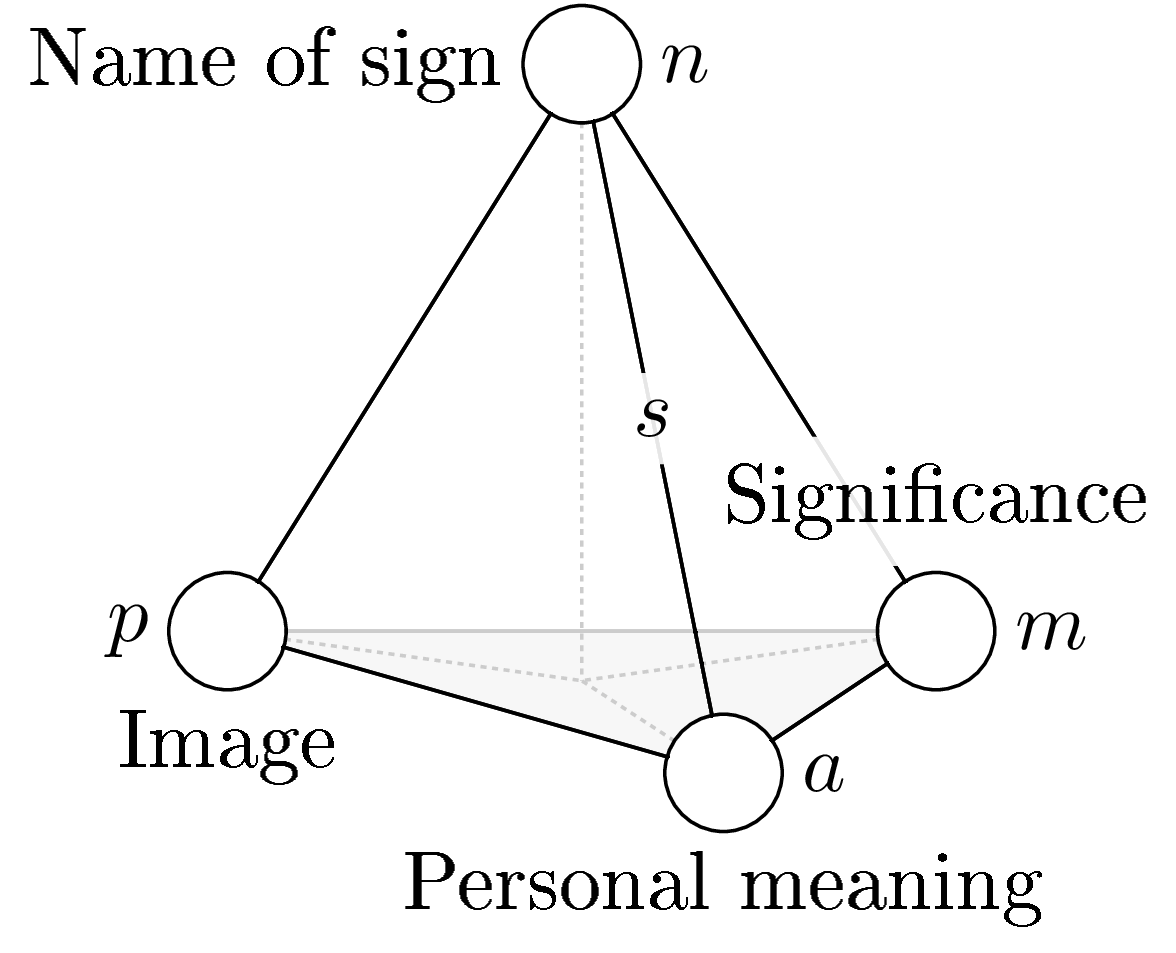
\includegraphics[width=0.5\textwidth]{sign_eng-0.png}
	\caption{Structural components of the element of the world model.}
	\label{fig:sign}
\end{figure}

The three-component structure of individual knowledge, which, as mentioned above, is called the sign in psychology and confirmed by the work of neuroscientists, is an attempt to construct a general theory of operation of the human brain. Thus, in the re-entry theory of Edelmena \cite{Edelman1987} and Ivanitsky \cite{Ivanitsky1996} it is approved that the formation of conscious sensation or fixing input flow occurs only when the excitation has been activated by sensory input via the associative cortex from the hippocampus, and then imposed on the sensory track on the projection cortex from hypothalamus. This ``circle of sensations'' that passes over a characteristic time in the 150-300 ms sequentially activates the three components of individual knowledge: the image (primary and sensory cortex), the significant component (hippocampus) and the personal meaning (the hypothalamus). In addition, the structure of the cerebral cortex, based on modern neurophysiological concepts, is almost uniform in its entirety (the existence of neocortical columns). Hereby the plurality of links between small enough areas of the cortex (the so-called connectome \cite{Zador2012}) clearly indicates its hierarchical structure and the presence of both uplink and back downlink. It follows that the components of individual knowledge elements should have a hierarchical homogeneous structure with ascending information flows and descending feedback. Furthermore, the significant component should have such recognition function, except for the categorization of static objects and dynamic processes, which uses a feedback signal for predicting a sign the next time.

Presented knowledge representation on the strategic level has common points with existing works in this area. So, an approach that can be represented in terms of ``heterogeneous proxytypes'' \cite{Lieto2014} should be noted. Knowledge base contains heterogeneous pieces of information semantically pointing to the same object and conveying different types of information. Such pieces of information may be contextually activated by an agent according to the external stimulus being categorized. In these categories we can also describe partitive information communication between agents but cannot get grounding in other levels of knowledge representation.

To define the mathematical model of components of individual knowledge elements infinite state machine with variable structure and finite memory (recognizing state machine or R-SM):
\[
	R_i^j =\langle X_i^j \times \hat X_i^{j + 1}{,2^{{\cal Z}_i^j}},X_i^{*j} \times \hat X_i^j,\varphi _i^j,\vec \eta _i^j\rangle,
\]
where $i$ --- the index of R-SM through the hierarchy, $j$ --- the level of the hierarchy, $X_i^j$ --- the set of input signals, $X_i^{*j}$ --- the set of output signals, $X_i^{j+1}$ --- the set of control signals from the upper layer of the hierarchy, $\hat X_i^j$ --- the set of control signals to the lower layer of the hierarchy, ${2^{{\cal Z}_i^j}}$ --- the set of states (Boolean of prediction matrices (see below)), $\varphi _i^j:X_i^j \times \hat X_i^{j + 1} \to {2^{{\cal Z}_i^j}}$ --- the transition function, $\vec \eta _i^j:{2^{{\cal Z}_i^j}} \to X_i^{*j} \times \hat X_i^j$ --- the vector-function of outputs. Input, output and control signals are vectors of real numbers. Each component of these vectors is a weight of recognizing or input feature.

As a recognition function ${\hat f_k}$ of the $k$ the output feature in R-SM it is convenient to use the set of bit prediction matrices ${Z_k} = \left\{ {Z_1^k,Z_2^k, \ldots ,Z_m^k} \right\}$. In these matrices each column $\bar z_u^r$ is the prediction vector of input features in the moment ${\tau _s} + u$, where ${\tau _s}$ is a start of the calculation circle (the moment of operation of the control signal $\hat x_i^{j + 1}$). The matrix $Z_r^k$ specifies the sequence of bit vectors where each bit indicates presence of a feature recognized by the function ${\hat f_k}$. The algorithm ${\mathfrak A}_{th}$ that calculates the transition function $\varphi _i^j$ and the vector-function of outputs $\vec \eta _i^j$ by the initial moment ${\tau _s}$, the control effect $\hat x_i^{j + 1}\left( {{\tau _s}} \right)$ and the input effect $\omega _i^j$ is shown on \autoref{fig:rfs}.

\begin{figure}[h]
	\centering
		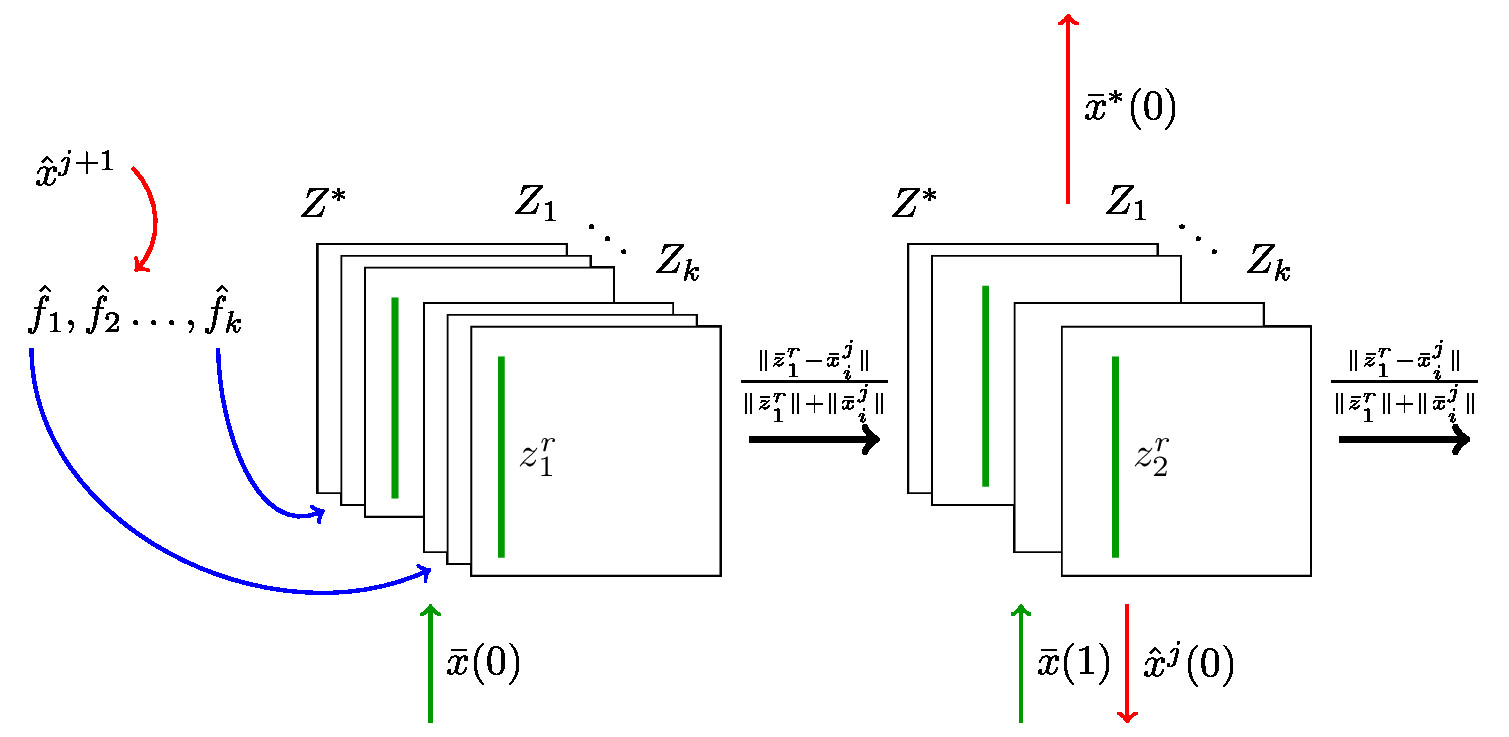
\includegraphics[width=\textwidth]{alg_th_schema.jpg}
	\caption{Schema of the R-SM's function. From the set of measure functions $\hat F_i^j$ subset is selected by prediction vector ${\hat x^{j + 1}}$ entering from the upper level. This subset of active functions forms the set of active prediction matrixes $Z^*$. This subset is filtered on each time step according to the input vector ${\bar x^j}$ and the simple distance metric. On each time step the output vector ${\bar x^*}$ and prediction vector ${\hat x^j}$ into the lower level are constructed.}
	\label{fig:rfs}
\end{figure}

Introduction of that R-SM and several relationships on the set of R-SM allows defining all components of the sign. The image of the sign $s$ corresponding to the feature ${f_1}$ is a subset $p(s)$ of features where $\forall f_i\in p(s) f_i\sqsubset f_1$. Here the relationship $\sqsubset$ is the relationship of subsumption of one feature by another. If the set of columns of a prediction matrix is divided into two subsets, columns of conditions and columns of effects, then each feature that has such prediction matrices is named as a procedural feature. If ${f_1}$ is a feature corresponding to the sign $s$, $f_2$ is a procedural feature and $f_1 \sqsubset^c f_2$ then $f_2$ is named as an element of significance of $f_1$. If $F_I$ is the subset of features where each feature describes characteristics of the control system then the definition of personal meaning will be as follows: $f_1$ --- the feature corresponding to the sign $s$; $\sqsubset$ --- the procedural feature, $f_1 \sqsubset^c f_2$, $\exists f_I\in F_I: f_I \sqsubset^c f_2$, $f_2$ is named as an element of personal meaning of $f_1$.

The proposed approach to the description of the image component of the sign using state machine representation has been applied to the wire toy recognition task. The input dataset for this task contains sequences of shifted wire toy pictures comprising of variations of eight types of figures (see \autoref{fig:htm_exp}). Hierarchy of R-SM contains three-level counting simple Bayes classifier on the highest level. On the lowest level of the hierarchy the set $X_i^j$ of the first R-SM was presented by a sequence of vectors, each component of which represented the gray scale value of the corresponding pixel of the input image. The set $X_i^{*j}$ of the R-SM was the set of vectors of which each component was the likelihood of a presence of memorized patterns on the parts of the image. The set $\hat X_i^{j + 1}$ contained predicted patterns at the next time from the second layer. On the next level, R-SM encoded a sequence of patterns for the corresponding part of an image consisting of several pixels. The top-level Bayes classifier took the decision about the name of the input sign. \autoref{fig:htm_exp} depicts the schema of the experiment, test images and accuracy of recognition, dependent on the level of noise on the image.

\begin{figure}[h]
	\centering{
		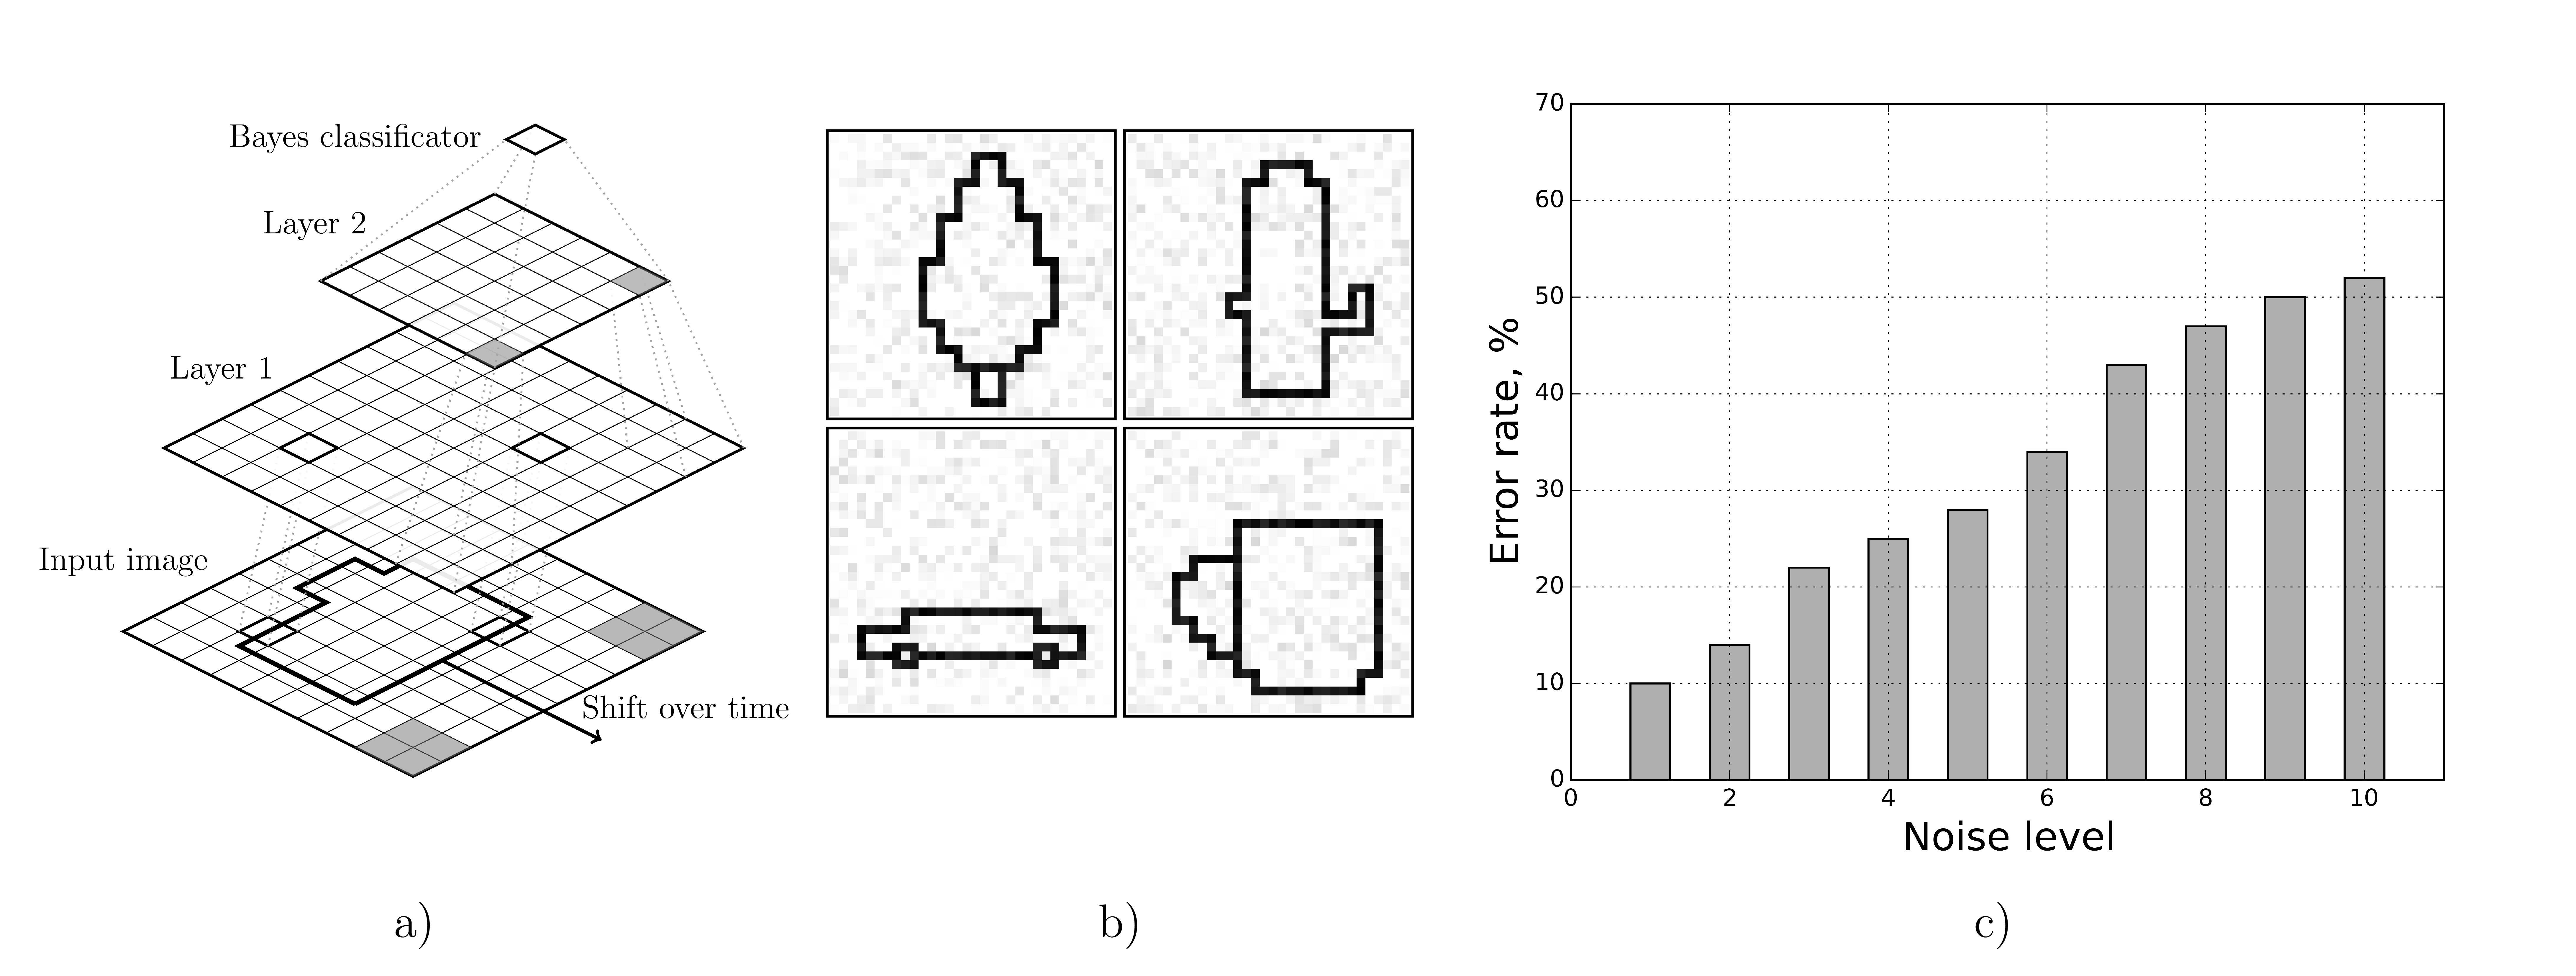
\includegraphics[width=\textwidth]{test_rita-0.png}
	}
	\caption{Experimental results of R-SM recognition tests. a) a schema of R-SM hierarchy used in the task, b) --- an example of test images with noise, c) --- accuracy of recognition, dependent on the image noise level.}
	\label{fig:htm_exp}	
\end{figure}

\subsection{Self-organized processes}
Within the process of the actor activity specific relationships occur on the sets of sign components. In its turn it leads to the formation of the world model of the UAV. Three types of semantic networks were used as a model of the UAV's knowledge about the world. These are the network based on the set of sign images, the network based on the set of sign significances and the network based on the set of personal meanings. Self-organized processes on these networks involve the supplementation of the relationships' collection as well as the formation of new nodes of the network, which corresponds to the formation of a new element of individual knowledge.

The process of the formation of a new sign includes establishing connections between the sign components and the naming generation structure. Until the name is obtained, this structure is called a protosign and its components are called percepts (evolved into the sign image), a functional significance (evolved into the sign significance), and a biological meaning (evolved into the personal meaning after the sign formation completion). Common schema of a new sign formation \cite{Osipov2014}
\begin{enumerate}
	\item\label{ph_1} The formation of a percept.
	\item\label{ph_2} Generation of the set of pairs ``percept---functional significance'' of the functional significance of the object based on the previous experience or precedents.
	\item\label{ph_3} From the cultural environment based on the external collective information objects (for example, texts) the actor obtains the pair ``sign name---significance'', accumulated in the natural language system, and evaluates the degree of closeness of the functional significance obtained in the phase~\ref{ph_2} to the significance obtained from the cultural environment. If these significances are not close enough, then the percept formation continues by returning to phase 1.
	\item\label{ph_4} Linking the name from the pair ``sign name---significance'' to the percept constructed after the completion of phases~\ref{ph_1}--\ref{ph_3}. At this time, the percept turns into an image.
	\item\label{ph_5} Formation of personal meanings of the sign based on precedents of actions with the object.
	\item\label{ph_6} Linking the name from the pair ``sign name---significance'' to each personal meaning. From this time on, the functional significance turns into the significance, and the biological significance turns into the personal meaning.
	\item\label{ph_7} Continuing to map the biological significance---percept by including the personal meaning (formed in the preceding phase) in the domain and by including the image formed in phase~\ref{ph_4} in the set of values.
\end{enumerate}

Consideration of procedural features in the form of rules with defined sets of added and removal features allows algorithm construction of the main iterative process (phases~\ref{ph_1}--\ref{ph_3}) of the described sign formation schema with R-SM. To define conflictness and applicability properties of rules on the set of procedural features special operations are introduced. These are the cast of the column $\bar z$ to the R-SM $R$($\bar z \to R$) and the cast of the column $\bar z$ to the R-SM $R$ by the column $\bar z$ ($\bar z\mathop  \to \limits^{{{\bar z}'}} R$).

\section{Details of organization on tactical level}\label{sec:tactical}
The tactical level lies in between a strategic level and a reactive level and serves as a bridge which connects high-level, intelligent activities (cognitive world modelling and behaviour generation) with the low-level ones aimed at forming control signals needed to operate the UAV and perform flight maneuvers. Our main idea is that both of these classes of activities can be meditatively connected via the spatial world model. The strategic level can output the time-spatial reference (associated with some high-level task the UAV has to perform) as an input to the tactical level modules. At the same time the reactive level is able to transform the model of UAV dynamics constraints into spatial models of constraints (either geometry or metric or, as we propose, both) and provide them to spatial planners residing on the tactical layer. In that case the core activity of the tactical level (which is the main mediator within the architecture) is to maintain the process of spatial reasoning. The latter is split into three main sub-processes: localization --- registering the state of the UAV in the respect to the spatial world model (SWM); mapping --- maintaining the consistency of the spatial model of the world; and path planning --- finding a sequence of states of the SWM ending with the goal state provided from the strategic level.

In modern robotics and AI the first two abovementioned processes are usually tied together in what is called simultaneous localization and mapping (SLAM). There exist dozens of methods and algorithms nowadays to solve the SLAM task, each of which differs from the others mainly in the input data it can process (but not in the way it processes these data). The input data include at least the following components: a mathematical model of UAV dynamics and the sensory data. So, practically speaking, different SLAM methods are needed for different robotic systems (as different robotic systems are equipped with different types of sensors and have different dynamic models). If we narrow ourselves to the vertical take-off and landing of multirotor UAVs (multicopters), the following SLAM algorithms can be named. First of all, if the UAV is equipped with laser range-finder SLAM algorithms, initially developed for ground robots, these can be used successfully (with some modifications); see \cite{Borrmann2008} for example. When the stereo-camera is used, the SLAM algorithms based on the computational geometry and computer vision are used \cite{Sim2005}. If the UAV is equipped only with a single (forward-looking camera), then such methods as \cite{Saxena2007,Bills2011} can be used. Needless to say, in many cases there exists a prior map which is also an input to the SLAM algorithm, so that mapping is often not meant to be the process of building the spatial world model from scratch (although it can be so) but of updating and refining it. Also, in some cases a localization task becomes trivial; for example, when the UAV is performing outdoor flight and is equipped with global positioning sensors (GPS receivers).

Path planning methods may be presumed to be more universal than the SLAM ones as they do not deal directly with sensor data. In effect, one path planning algorithm can be used for many different types of robotic systems. Typically the input to the path planning module (method) is the spatial world model (along with the references to the desired goal state(s) and current start state), and that is the case within our architecture. Usually, the spatial world model is a graph where each node corresponds to some 3D (or 2D) point (location) and each edge corresponds to so-called elementary trajectory (typically the segment of a straight line). This is a trajectory that can be followed in a reactive way by the use of lower level methods and algorithms --- the modules of the reactive level of the control system --- so that path planning is viewed as a graph search \cite{Likhachev2008}.

In our work, we assume that 3D (or 2D) grid \cite{Yap2002} is used as the spatial world model as it is a simple and powerful graph model successfully used both in ground \cite{Elfes1989} and aerial robotics \cite{Filippis2012}. Grids are so widespread because they can be extracted from the output of the SLAM module(s) by naive, fast and efficient algorithms (in most cases only post-processing is done). To find a path on a grid, one can use one of the numerous algorithms of heuristic search: A* \cite{Hart1968}, R* \cite{Likhacjev2008}, JPS \cite{Harabor2011}, Theta* \cite{Nash2007} etc. The main problem here is that the result --- path found as the sequence of free grid cells and sections --- is not guaranteed to be executable by the lower level of the control stack, i.e. corresponding control signals to follow the path cannot be generated. The most obvious example of such a path is a path containing a sharp turn when the corresponding maneuver cannot be performed due to the vehicle's dynamics constraints. One way to take these constraints into account is to extend the graph model used to search for a path. In that case we are talking about finding a path as a sequence of states which are referred not to the elements of spatial world model but to the elements of some extended graph model which incorporates also information on UAV dynamics. As an example of the algorithm exploiting such an idea one can name \cite{Kuwata2009,Kothari2013}.

As mentioned above, one of the core intuitions which underlies the proposed architecture of the control system is that the reactive level of control can be separated from higher levels and, for this, we are proposing the mechanism of such separation is to find a model of geometry constraints which can easily be incorporated into the spatial world model, on the one hand, and take into account UAV dynamics, on the other. We propose the following model of geometry constraints: we assume that the executable trajectory corresponds to the grid path which can be presented as the sequence of such sections that the angle in between each pair of them does not exceed predefined threshold $\alpha_m$. On \autoref{fig:angles} two paths are depicted: the one on the left violates maximum level of alteration constraints and the one on the right does not.

\begin{figure}[h]
	\centering
		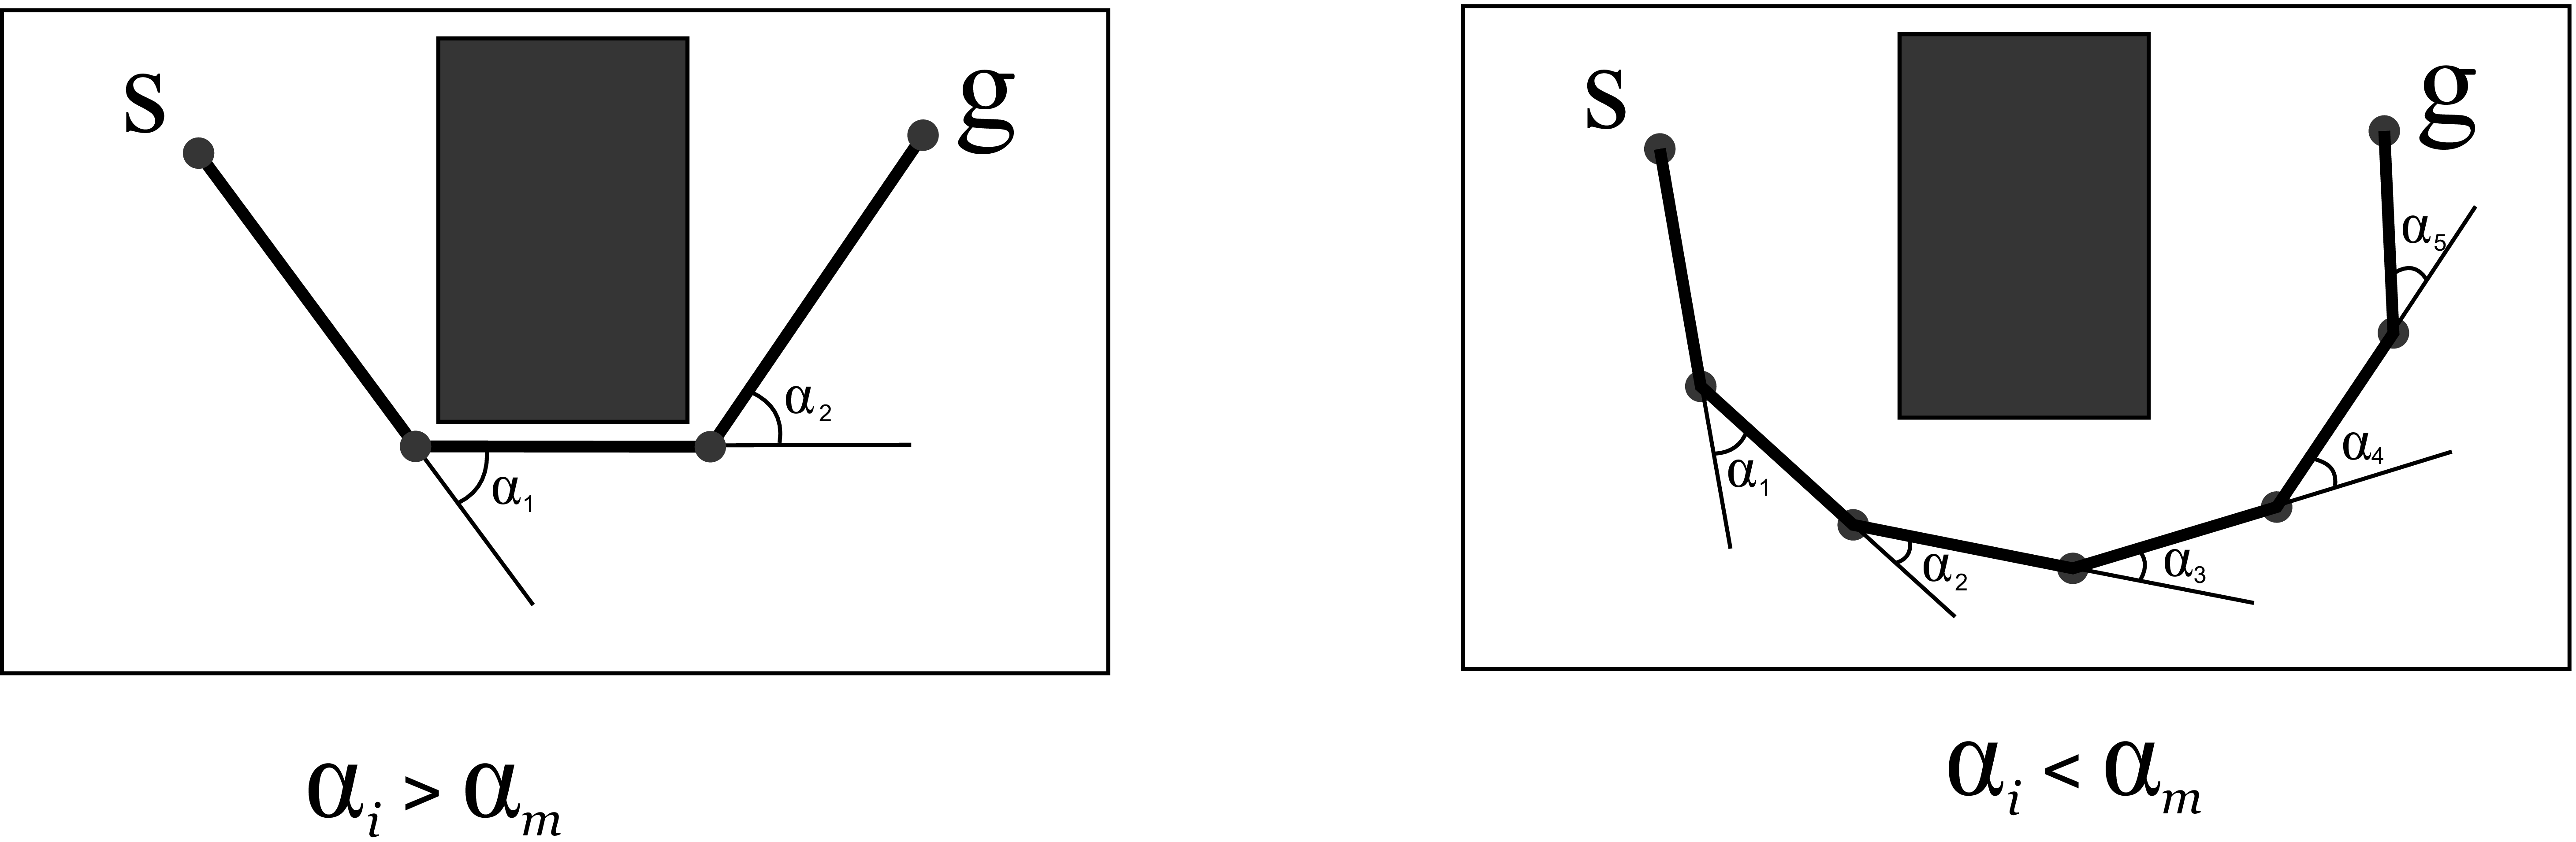
\includegraphics[width=\textwidth]{path_lian.png}
	\caption{Angle constrained path (on the right) and a path violating maximum angle of alteration constraint (on the left).}
	\label{fig:angles}
\end{figure}

The exact value of the threshold --- $\alpha_m$ --- is estimated by the module which resides at the reactive level and takes into account all constraints imposed by the vehicle dynamics, control laws, etc. For more detail, the method of the constraints transformation is described in \autoref{sec:reactive} of this paper.

To the best of the authors' knowledge, there are not many grid path planning methods capable of taking angle-change constraints into account, although methods based on similar ideas of constraints modelling do exist (see \cite{Kim2014} for example). Thus, we have developed and studied both theoretically and empirically a new path planning method for the proposed model of geometry constraints --- LIAN (from ``limited angle''). It is pretty similar to a classic A* search as it uses the same heuristics and strategies to focus the search. The main difference is that at each step A* is investigating only grid cells that are immediate successors of the current one (i.e. they are adjacent to the current one) while LIAN ``jumps'' to the cells that lie at some distance from the current cell (exact distance value --- $\Delta$ --- is an input parameter of the algorithm). By doing this we implicitly present each partial path (in the set of all paths under investigation) as the sequence of sections. Thus, paths which do not satisfy ``in-between-section angle'' constraint are easily pruned. It is proved that the proposed algorithms are sound and complete (with respect to the input parameter $\Delta$). More details on the proposed algorithm can be found in \cite{Yakovlev2015a,Yakovlev2015b}.

An example of the path generated by the proposed algorithm can be seen in \autoref{fig:grid}. The start cell is located on the left edge of the grid and the goal is located on the right. The path is shown as a curved line. Cells that have been visited by the algorithm (so called OPEN and CLOSE lists in heuristic search literature) are shaded in light grey. Obstacles are shaded in dark grey. One can clearly see the ``jumps'' as the caverns of unvisited cells in between the visited ones (centre and right of the picture). The most explored area is located on top of the left-most obstacle: LIAN has investigated a handful of variants of passing that obstacle, in such a way that the maximum angle of alteration constraint is not violated, before finally finding a suitable path fragment.

\begin{figure}[h]
	\centering
		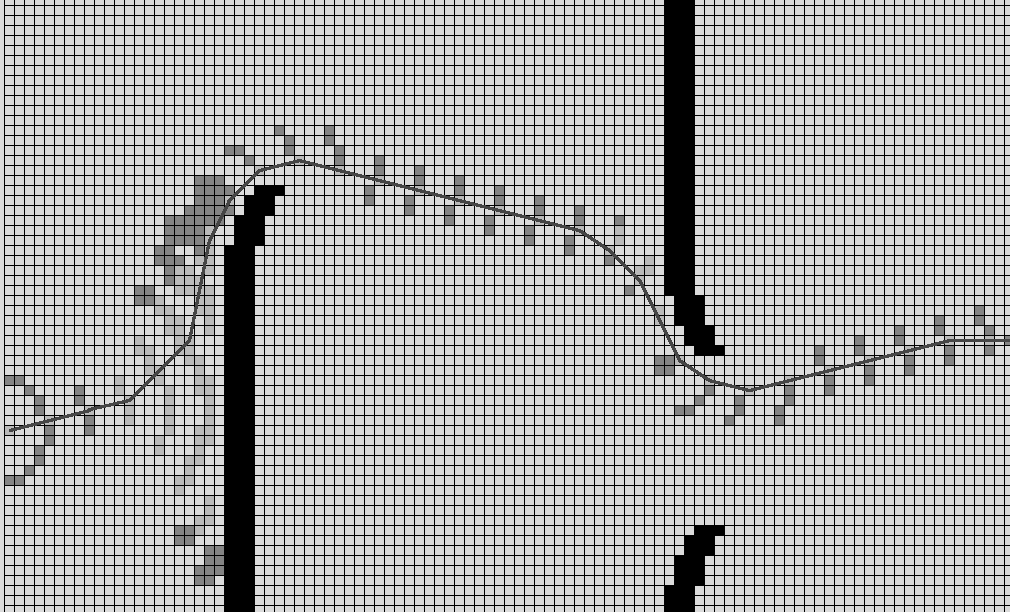
\includegraphics[width=\textwidth]{fig6.png}
	\caption{The path found by the LIAN algorithm as well as the explored areas (shaded in light gray).}
	\label{fig:grid}	
\end{figure}

We have conducted an empirical study of LIAN and compared its ability to solve angle-constrained path planning tasks and it’s performance to the competitors: naïve modification of Theta* which takes into account angle constraints --- Theta*-LA; and its modification implementing grid-weighting techniques --- wTheta*-LA (for the original description of algorithms see \cite{Kim2014}, for the details of author’s implementation of algorithms and experimental setup see \cite{Yakovlev2015b}). We have used 80 different fragments of city maps (retrieved from OpenStreetMaps \cite{OpenStreet} database) sized 1347m x 1347m each and discretized to 501x501 grids, and we have chosen 5 different start-goal locations on each grid. Various angle constraints were targeted. For example $\alpha_m=25$ corresponds to AscTech UAV flying at the air speed of 7 m/s, the typical cruise speed in urban environments. Results are shown in the \autoref{tab:lian_res}.

\begin{table}
	\caption{Comparative study of LIAN, Theta*-LA and wTheta*-LA path planning algorithms.}	
	\label{tab:lian_res}\scriptsize
	\centering{
		\begin{tabular}{c|ccccc|ccccc}
			&\multicolumn{5}{c|}{$\alpha_m=25$}&\multicolumn{5}{c}{$\alpha_m=30$}\\
			&$sr$&PAR-10&$t$&$m^*$&$pl$&$sr$&PAR-10&$t$&$m^*$&$pl$\\
			\hline
			LIAN-5&98\%&12&0.5&6.3&1617&98\%&11&0,5&6.1&1611\\
			Theta*-LA&12\%&536&2.1&37.5&1574&31\%&421&2.2&47.4&1580\\
			wTheta*-LA&55\%&277&2.76&58.3&1598&73\%&165&2.7&61.0&1567\\
		\end{tabular}
	}
\end{table}

Here $sr$ (success rate) is the number of accomplished angle-constrained path planning tasks divided by the number of all tasks (time limit for each task was set to 60 seconds); PAR-10 (penalized average runtime) is the metric that averages the runtime and takes failures into account \cite{Hutter2009}; $t$ (time) is the time (in seconds) needed for an algorithm to produce solution averaged without taking failures into account; $m^*$ (memory) is the number of intermediate grid elements explored by the algorithm and stored in memory (the memory consumption of the algorithm); $pl$ is the length (in meters) of the resulting angle-constrained path.

Results of the experiments prove that the proposed algorithm significantly outperforms existing analogues (at least for the considered outdoor navigation scenarios): LIAN solves more angle-constrained path planning tasks than the competitors while using less memory and processing time. In \cite{Yakovlev2015b} the reader can find more details on the algorithm’s experimental assessment. 

In order to form a geometrical model of the executable trajectory constraints, modules of the reactive level need to be provided with the input that defines the values of basic UAV movement parameters (for example --- speed). To calculate these parameters, a path prediction module residing on the tactical level is used. Basically path prediction can be considered as fast, constraint-free version of path planning. In the simplest case, when the goal location and time of the arrival is received from the higher level, the length of the straight line connecting the current UAV location and the goal is calculated and used to determine the desired (minimum) speed of traversal, which is then passed to the ``geometry model generation'' module of the reactive level. Furthermore, with such a straightforward computation more complex algorithms can be used (for example, path planning algorithms utilizing over-informative heuristics or taking no spatial constraints (obstacles) into account).

The last module of the tactical level not described so far is a path monitoring module. It receives the current location of the UAV and matches it up with the planned path. If the discrepancy exceeds a predefined threshold it triggers again the ``path prediction --- geometry constraints generation --- path planning'' loop to find a new path to the goal state. If such a path cannot be found, the corresponding module at the strategic level of the control system is informed, and the global goal-change process is triggered). 

\section{Details of organization on reactive level}\label{sec:reactive}
As already noted, the main challenge for the reactive level is to provide specified dynamic object characteristics (speed, location, etc.), received from the tactical level, by the means of a control signal generated by the controller. The control signal is applied to the UAV actuators: screws engines, ailerons, etc. Additionally, using the appropriate procedure, the problem of calculation of geometric constraints on the admissible trajectory of movement is solved at this level. Let us describe the methods of controller synthesis and constraints calculation that are proposed in our architecture.

\subsection{Method of controller synthesis}
In the area of automatic control there are many approaches and techniques to the construction of the controller. Some of them are indirectly related to a cognitive human activity at the level of implementation and control of motor actions. For example, the control based on artificial neural networks (ANN) uses the principle of learning by examples, and control based on fuzzy logic uses the formalized intuitive knowledge of domain experts. The application of these techniques is particularly useful if there is no possibility to build an adequate mathematical model of UAV. A few works on the use of ANN and fuzzy logic to automate the UAV's flights are outlined in \cite{Garcia2009,Buskey2001}. The main disadvantage of the noted approaches is the lack of a rigorous proof of operability of such controllers. On the other hand, there are many rigorous techniques free from this disadvantage that do not rely on human motor activity, such as the synthesis of linear-quadratic controller, H-infinity methods, feedback linearisation, backstepping methodology, etc. Limited area of application is a disadvantage of such techniques: they deal with either a linear model of the UAV or a nonlinear model of a special kind.

In the proposed architecture one of the promising approaches used is based on the Riccati equation with state-dependent coefficients (SDRE --- State Depended Riccati Equation). Work in this area has been carrying out actively since the mid-90s of the last century \cite{Mracek1998,Cimen2008}. On the one hand, development and application of this technique provide a fairly general methodology for constructing suboptimal, smooth, nonlinear, state dependent controllers for nonlinear systems. On the other hand, the SDRE control allows us to use some of the principles that are utilized in the realization of lower cognitive human functions, associated with the control and execution of motor actions. Namely, it is possible to adapt the control signal depending on the mode and conditions of operation, and constraints on the control. Let us describe the approach.

The SDRE technique is based on the representation of the original nonlinear system in the quasi-linear form. This allows us to apply the procedure for stabilizing control constriction similar to a procedure for optimal synthesis for linear systems (linear-quadratic regulator synthesis) by means of considering the corresponding algebraic Riccati equation, whose coefficients are already dependent on the state variables of the original system. 

The Riccati equation, as in the linear case, is given by the linear quadratic cost functional, reflecting the quality requirements of the transition process by entering two weight matrices, for state and control. The objective of control is to minimize the functional. However, the elements of these two matrices are also non-linear functions of the state. This fact allows the specification of different requirements for the transition process, depending on the operating mode of the system (areas of phase space), as well as taking into account the existing control constraints. For example, the requirements for the trajectory accuracy is to be increased at the final stage of a missile flight or at aircraft landing, so that values of the respective elements in the weighting matrix of the system state increases to modify the control law. Besides, one can modify a control weight matrix to create an area in a state space, where the gain should be lowered because of the probability of the control saturation.

Thus, the controllers synthesized in this way can compensate nonlinearity of control systems by means of the SDRE numerical solution, taking into account \cite{Cloutier2001,Cloutier2002} constraints both on control and the system state, and can continuously change their algorithm depending on the scenario of the task.

In contrast to the well-known linear-quadratic regulator synthesis, the SDRE technique requires real-time performing of a number of quite computationally difficult operations to solve the matrix Riccati equation for each of the current states of the system. This may require significant computational resources. Technically it can be realized only with a certain time step, varying depending on the computational complexity of a particular problem-solving task. 

To overcome this difficulty, the authors proposed an original method for the approximate analytical solution of SDRE, which significantly reduces the required computations. The asymptotic stability of the resulting control system can be rigorously proved by means of Lyapunov function. 

The performance of proposed method was confirmed by the ``classical'' task of stabilizing a nonlinear second-order system: the inverted pendulum from paper \cite{Dutka2005}.  Constructed nonlinear control is up to 70\% more effective on the considered quadratic cost function than linear control, which is optimal at the equilibrium point of the system. However, the experiments showed that the nonlinear control effectiveness significantly depends on the initial conditions. It decreases when the initial conditions tend toward the equilibrium point of the system. In a small neighbourhood of equilibrium point linear control, even slightly better (up to 10\%) results are produced than in a constructed nonlinear one. In general, the estimation of proposed analytical solution accuracy is the subject of the further investigations.

Thus, in our architecture we use the algorithm for constructing a nonlinear controller, which greatly reduces the amount of computation compared with traditional procedures of the SDRE control approach. Another distinctive feature of the approach is sufficient mathematical and rigorous proof of closed system stability, as well as the opportunity to use some principles which affect human motor actions: it is possible to adapt the control signal depending on the mode and conditions of operation and constraints on the control. More details on the proposed method can be found in \cite{Dmitriev2014}.

\subsection{Method of constraints calculation}
In the case of horizontal flight, the tactical level algorithms are trying to construct a trajectory in the form of a straight line sequence in which the angle between any adjacent lines of the sequence does not exceed (in absolute value) a fixed value α. It is assumed that satisfaction of this condition ensures the feasibility of the resulting trajectory, i.e. the possibility of constriction of an admissible control signal to follow the trajectory with the specified error. The proposed method of geometric constraints calculation is based on numerical analysis of an attainability domain of a dynamic system. The exact solution of this problem usually requires a large computational cost. Let us confine ourselves to a simplified approach based on certain plausible assumptions. Nevertheless, the proposed approach is rather general for a lot of applications. 

Let us suppose that a UAV must follow the trajectory tr. Our basic assumption consists in the idea that the flight conditions and precise control within its constraints make it possible to construct admissible control, which guarantees that the UAV is located in some admissible neighbourhood of the desired straight-line trajectory. This neighbourhood is defined by the ``tube'' with a radius $r_d$ (see \autoref{fig:geometr}). The specific value of rd depends on the type of UAV, conditions and mode of flight etc. It is assumed that values of rd are known (e.g. based on the operating experience of the selected UAV).

\begin{figure}[h]
	\centering
		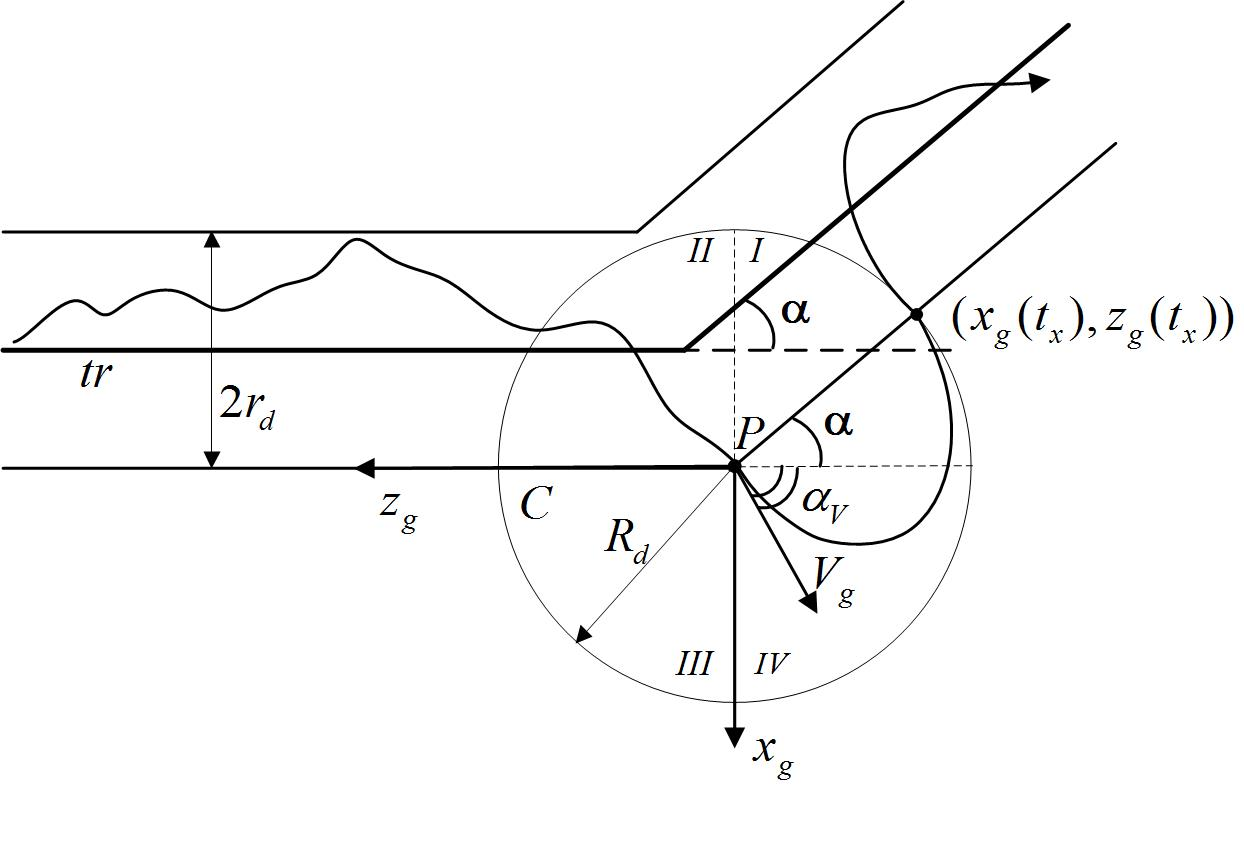
\includegraphics[width=\textwidth]{ang_plan.jpg}
	\caption{To the method of geometric constraints calculation.}
	\label{fig:geometr}	
\end{figure}

Obviously, in the case of trajectory breaking, shown in \autoref{fig:geometr}, the location of the UAV at the point $P$ did not belong to the ``tube'', which is the worst challenge for control. Let us consider an additional area to be defined by a circle $С$ with a given radius $R_d$ and to be centred at the point $P$. It is assumed that any point in $С$ does not contain obstacles. In fact, the radius $R_d$ determines the turning maneuver area. 

It is assumed also that in the worst case, which is considered below, the velocity vector $V_g$ of the UAV is deflected from desired flight trajectory before breaking in the point $P$ at a maximum angle $\alpha_v$ (see \autoref{fig:geometr}). Then the problem of geometric constraints calculation may be formulated as follows. It is necessary to find the maximum angle $\alpha$, so that the UAV trajectory, without leaving the circle $С$, will return again in the admissible ``tube'' and will no longer leave it (because of the basic assumption above, there is always an admissible control which guarantees it).

Next, it is assumed that $R_d$ value is given (for example, by means of location map analysis) and the value of the velocity $V_g$ is supplied as a parameter from the tactical level. Besides, it is assumed that the maximum of the UAV allowable control is applied. Let axis $Ox_g,Oz_g$ of Earth coordinate system $Px_gy_gz_g$ to be oriented as shown in \autoref{fig:geometr}, and the axis $Oy_g$ is oriented vertically upward. Then the following algorithm for angle $\alpha$ determination is correct. 

Make a numerical simulation of the UAV motion dynamics, starting at the point $P$ with the velocity $V_g$, up to the time $t_x$ at which one of the following conditions holds:
\begin{enumerate}
	\item The trajectory crosses the circumference corresponding to circle $C$ in sector I or II. Then using the geometric considerations (see \autoref{fig:geometr}), one may calculate the desired angle by the formula
	\[
	\alpha (t)=\arccos \left( \frac{-{{z}_{g}}({{t}_{x}})}{\sqrt{{{x}_{g}}{{({{t}_{x}})}^{2}}+{{z}_{g}}{{({{t}_{x}})}^{2}}}} \right),
	\]
	where ${{x}_{g}}({{t}_{x}}),{{z}_{g}}({{t}_{x}})$ represents UAV coordinates in $Px_gy_gz_g$ at time $t_x$.
	\item The trajectory crosses the circumference corresponding to the circle $C$ in the sector IV. This case means that under the current flight parameters the UAV does not have time to make the maneuver, and the angle $\alpha=0$. It is necessary to change the flight parameters or expand the area of the maneuver, i.e. increase the $R_d$ value.
	\item The trajectory comes to the sector III, passing through the sectors I and II. This means that $180^\circ\leq\alpha\leq 270^\circ$ for both given flight conditions and $R_d$ value, i.e. geometric constraints are absent. It is necessary to decrease the $R_d$ value.
	\item The maximum simulation time is reached. It corresponds to the case when the UAV behaviour dynamics are rather complicated: the trajectory does not leave sectors I, II or IV of the circle $C$. For sufficiently larger simulation time it may be concluded that the restrictions on geometry of the trajectory are also absent. It is necessary to decrease the $R_d$ value.
\end{enumerate}

The proposed method was tested for the mathematical model of the AscTec Hummingbird quadrocopter \cite{AsTec}. Results for different flight conditions and $\alpha_v=45^\circ$ are shown in \autoref{tab:react_res}.

\begin{table}
	\caption{Calculated angle $\alpha$ for for different flight conditions.}	
	\label{tab:react_res}\scriptsize
	\centering{
		\begin{tabular}{c|c|c}
			$R_d$,m&$V_g$,m/s&$\alpha$,$^\circ$\\
			\hline
			2.7&6.5&$\alpha\geq 180$\\
			2.7&6.9&31.7\\
			2.7&7&24.4\\
			2.7&7.5&7.8\\
			2.7&8&0\\
			5.4&8.5&$\alpha\geq 180$\\
			5.4&9&34.5\\
			5.4&9.5&17.5\\
			5.4&10&0\\
		\end{tabular}
	}
\end{table}

Thus, a quite general method of geometric constraints calculation is proposed. It's based on the model of a flight dynamics, as well as some plausible assumptions. The method can be improved by taking into account the external disturbance, such as wind (see the paper \cite{Yakovlev2015a} for details).

\section{Conclusion}\label{sec:concl}

One of the obvious recent trends in science and technology is the rapid growth of the R\&D areas related to UAV design. UAVs themselves are getting cheaper and thus more available both to researchers and the general public. Nowadays there exist numerous unified, moderately priced UAV platforms equipped with all the needed hardware and software to perform basic flight maneuvers. Typically this software provides seamless integration of third-party modules, which has lead to the currently observed situation, in which a lot of research is focused on the development of methods and algorithms for existing UAV platforms (rather than creating UAVs from scratch). 

Thus, the direction of research that has a great importance now is studying the methods of interaction between the modules of control systems and the ways of organizing hierarchical relations between them. That is to say, studying and developing the architectures of modern UAV intelligent control systems. Such intelligent control systems are able to solve non-trivial, intelligent tasks such as planning, goal prioritization, coalition formation etc. and thus guarantee high levels of autonomy for the UAV. 

We follow the cognitive approach and believe that the ability of the system to solve the abovementioned tasks relies on its ability to model human cognitive behaviour. We have proposed a multi-layered cognitive architecture --- STRL --- for the intelligent control system using cognitive experimental data and psychological methods. At the same time, the STRL-based control system is also meant to deal with the non-abstract technical objects (multirotor UAVs) and take complicated dynamics and kinematics of such objects into account.

Each module of the proposed architecture is supposed to solve some specified task(s) (the architecture can be referred to as explicitly specified) and the modules are grouped into levels which encapsulate the level of abstraction: the higher the level, the more abstract the representation of input signals it uses to solve a given task. The tasks being solved on higher levels of the system are considered more sophisticated and complicated than the tasks of the lower levels. We distinguish 3 levels of control and thus separate the following 3 levels within the architecture: strategic, tactical and reactive. 

The main task at the strategic level is to plan the behaviour of the single member (UAV) of joint activity and coordinate it with the other members of the coalition. The distinguishing feature of the proposed strategic level is the use of knowledge representation model based on neurophysiological and psychological studies of human cognitive functions: the sign world model. Such a representation allows us to construct sophisticated algorithms for coalition behaviour planning, goal-setting and communication. 

UAV navigation tasks are solved at the tactical level, which is the mediator between high-level activities with the low-level ones. The main distinguishing features of the tactical level are the utilization of spatial representation of the UAV dynamics constraints and the use of the following iterative loop to perform path planning: ``prediction'' --- ``calculation geometric constraints'' --- ``planning''.  We believe that such an approach (splitting planning into easily manageable stand-alone subroutines) would substantially improve the computational performance of the path planning process and thus improve the overall performance of the control system (as more navigation tasks will become solvable in the allotted time). 

The main challenge for the reactive level is UAV trajectory tracking control. Both desired trajectory and UAV speed are received from the tactical level. We use the approach of nonlinear control based on a special method of solving the state-dependent Riccati equation. It greatly reduces the amount of computation and increases the control accuracy.

We suppose that any intelligent control system that implements the proposed architecture will be capable of solving a broad range of tasks and will significantly raise the degree of autonomy of the control object. STRL architecture is especially tailored to the solution of the non-trivial, complex tasks when the role distribution and coalition behaviour planning is obligatory. The architecture provides a full stack of translation mechanisms: from high-level behaviour plans to spatial plans to control signals needed to follow these spatial plans (trajectories). The overall computational effectiveness of the control system implementing the proposed architecture relies on the use of the original methods of interaction between the planning modules residing on different levels of the STRL hierarchy.

\section{Acknowledgments}
This work was supported by the Russian Science Foundation (project no. 14-11-00692).

\section*{References}

\begin{thebibliography}{9}
	\bibitem{ArDrone} http://ardrone2.parrot.com/
		
	\bibitem{Bristeau2011} Bristeau P.-J., Callou F., Vissiere D., Petit N. The Navigation and Control Technology Inside the AR.Drone Micro UAV // Preprints of the 18th IFAC World Congress (Milano, Italy). Milano: IFAC. 2011. Vol. 18. Part 1. p. 1477-1484.
	
	\bibitem{mikrokopter} http://mikrokopter.de
	
	\bibitem{3dr} http://3drobotics.com/iris/
	
	\bibitem{Kendoul2012} Kendoul, Farid. ``Survey of advances in guidance, navigation, and control of unmanned rotorcraft systems.'' Journal of Field Robotics 29.2 (2012): 315-378.
	
	\bibitem{Albus2002} Albus, James S. "4D/RCS: a reference model architecture for intelligent unmanned ground vehicles.'' AeroSense 2002. International Society for Optics and Photonics, 2002.
	
	\bibitem{Kurup2012} Kurup U., Lebiere C. What can cognitive architectures do for robotics? // Biologically Inspired Cognitive Architectures. - 2012. - Vol. 2. - P. 88-99.
	
	\bibitem{Jameson2005} Jameson S., Franke J., Szczerba R., Stockdale S. Collaborative Autonomy for Manned/Unmanned Teams. AHS International Forum 61. Grapevine. TX. 2005.
	
	\bibitem{Gat1992} Gat, E. Integrating planning and reacting in a heterogenous asynchronous architecture for controlling real-world mobile robots. in National Conference for Artificial Intelligence. 1992.
	
	\bibitem{Bonasso1995} Bonasso, R.P., et al. Experiences with an Architecture for Intelligent, Reactive Agents. in International Joint Conference on Artificial Intelligence. 1995.
	
	\bibitem{Arkin1987} Arkin, R. Motor schema based navigation for a mobile robot: An approach to programming by behavior. in IEEE International Conference on Robotics and Automation. Proceedings. 1987.
	\bibitem{Anderson2004} Anderson, J. R., Bothell, D., Byrne, M. D., Douglass, S., Lebiere, C., \& Qin, Y. (2004). An integrated theory of the mind. Psychological Review, 111(4), 1036-1060. http://doi.org/10.1037/0033-295X.111.4.1036
	
	\bibitem{Langley2009} Langley, P., Laird, J. E., \& Rogers, S. (2009). Cognitive architectures: Research issues and challenges. Cognitive Systems Research, 10(2), 141-160. http://doi.org/10.1016/j.cogsys.2006.07.004
	
	\bibitem{Laird2012} Laird, J. E. (2012). The Soar Cognitive Architecture. MIT Press.
	
	\bibitem{Derbinsky2010} Derbinsky, N., \& Laird, J. E. (2010). Extending Soar with Dissociated Symbolic Memories. Proceedings of the Remembering Who We Are - Human Memory for Artificial Agents Symposium, AISB 2010, 31-37.

	\bibitem{Harnad1990} Harnad, S. (1990). Symbol Grounding Problem. Physica, 42, 335-346. http://doi.org/10.4249/scholarpedia.2373
	
	\bibitem{Barsalou1999} Barsalou, L. W. (1999). Perceptual symbol systems. The Behavioral and Brain Sciences, 22(4), 577-609; discussion 610-660. http://doi.org/10.1017/S0140525X99252144
	
	\bibitem{Osipov2014} Osipov G. S., Panov A. I., Chudova N. V. Behavior Control as a Function of Consciousness. I. World model and Goal Setting // Journal of Computer and Systems Sciences International. - 2014. - Vol. 53, no. 4. - P. 517-529.

	\bibitem{Leontiev2009} Leontiev A.N. The Development of Mind. Erythros Press and Media. 2009.
	
	\bibitem{Stanovich2009} Stanovich, K. E. (2009). Distinguishing the reflective, algorithmic, and autonomous minds: Is it time for a tri-process theory? In J. Evans \& K. Frankish (Eds.), In two minds: Dual processes and beyond (pp. 55-88). Oxford University Press. http://doi.org/10.1093/acprof:oso/9780199230167.003.0003

	\bibitem{Vygotsky1986} Vygotsky L. Thought and Language. MIT Press. 1986.

	\bibitem{Artemieva1999} Artemieva E. U. The bases of the psychology of the subjective semantics. / Edited by I .B. Khanina. Smisl, 1999. (in Russian).
	
	\bibitem{Edelman1987} Edelman G. M. Neural Darwinism: The Theory Of Neuronal Group Selection. - New York : Basic Books, 1987. - P. 400.
	
	\bibitem{Ivanitsky1996} Ivanitsky A. M. Brain basis of subjective experience: information synthesis hypothesis // Neuroscience and Behavioral Physiology. - 1996. - Vol. 46, no. 2. - P. 251-252.
	
	\bibitem{Zador2012} Sequencing the connectome / A. M. Zador, J. Dubnau, H. K. Oyibo et al. // PLoS biology. - 2012. - Vol. 10, no. 10.

	\bibitem{Lieto2014} Lieto, A. (2014). A Computational Framework for Concept Representation in Cognitive Systems and Architectures: Concepts as Heterogeneous Proxytypes. Procedia Computer Science, 41, 6-14. http://doi.org/10.1016/j.procs.2014.11.078
	
	\bibitem{Borrmann2008} Borrmann D., Elseberg J., Lingemann K., Nuchter A., Hertzberg J. Globally consistent 3D mapping with scan matching // Robotics and Autonomous Systems. 2008. Vol. 56, p. 130-142.
	
	\bibitem{Sim2005} Sim R., Elinas P., Griffin M., Little J. Vision-Based SLAM Using the Rao-Blackwellised Particle Filter // Proc. IJCAI-2005 Workshop Reasoning with Uncertainty in Robotics. 2005. p. 9-16.
	
	\bibitem{Saxena2007} Saxena A., Sun M., Ng A. Learning 3-D scene structure from a single still image // IEEE Transactions of Pattern Analysis and Machine Intelligence (PAMI). 2007. Vol. 30. no. 5. p. 1-8.
	
	\bibitem{Bills2011} Bills C., Chen J.,  Saxena A. Autonomous MAV flight in indoor environments using single image perspective cues // Proceedings of International Conference on Robotics and Automation ( Shanghai, China). 2011. p. 5776-5783.
	
	\bibitem{Likhachev2008} Likhachev, M., Ferguson, D., Gordon, G., Stentz, A., \& Thrun, S. (2008). Anytime search in dynamic graphs. Artificial Intelligence, 172(14), 1613-1643.
	
	\bibitem{Yap2002} Yap, P. 2002. Grid-based path-finding. In Proceedings of 15th Conference of the Canadian Society for Computational Studies of Intelligence, 44-55. Springer Berlin Heidelberg.
	
	\bibitem{Elfes1989} Elfes, A. 1989. Using occupancy grids for mobile robot perception and navigation. Computer, 22(6), 46-57.
	
	\bibitem{Filippis2012} De Filippis, L., Guglieri, G., \& Quagliotti, F. (2012). Path planning strategies for UAVS in 3D environments. Journal of Intelligent \& Robotic Systems, 65(1-4), 247-264.
	
	\bibitem{Hart1968} Hart, P. E., Nilsson, N. J., \& Raphael, B. 1968. A formal basis for the heuristic determina-tion of minimum cost paths. IEEE Transactions on Systems Science and Cybernetics, 4(2), 100-107.
	
	\bibitem{Likhacjev2008} Likhachev, M., \& Stentz, A. 2008, R* Search. In Proceedings of the Twenty-Third AAAI Conference on Artificial Intelligence. Menlo Park, Calif.: AAAI press.
	
	\bibitem{Harabor2011} Harabor, D., and Grastien, Al. 2011. Online graph pruning for pathfinding on grid maps. In 25th Conference on Artificial Intelligence (AAAI-11).
	
	\bibitem{Nash2007} Nash, A., Daniel, K., Koenig, S., \& Felner, A. (2007, July). Theta*: Any-Angle Path Planning on Grids. In Proceedings of the National Conference on Artificial Intelligence (Vol. 22, No. 2, p. 1177). Menlo Park, CA; Cambridge, MA; London; AAAI Press; MIT Press; 1999.
	
	\bibitem{Kuwata2009} Kuwata, Y., Karaman, S., Teo, J., Frazzoli, E., How, J. P., \& Fiore, G. (2009). Real-time motion planning with applications to autonomous urban driving. Control Systems Technology, IEEE Transactions on, 17(5), 1105-1118.
	
	\bibitem{Kothari2013} Kothari, M., \& Postlethwaite, I. (2013). A probabilistically robust path planning algorithm for UAVs using rapidly-exploring random trees. Journal of Intelligent \& Robotic Systems, 71(2), 231-253.
	
	\bibitem{Kim2014} Kim, H., Kim, D., Shin, J. U., Kim, H., \& Myung, H. (2014). Angular rate-constrained path planning algorithm for unmanned surface vehicles. Ocean Engineering, 84, 37-44.
	
	\bibitem{Yakovlev2015a} Yakovlev, K. S., Makarov, D.A., Baskin, E.S. (2015). Automatic Path Planning for an Unmanned Drone with Constrained Flight Dynamics. Scientific and Technical Information Processing, 42(5), 2015.
	
	\bibitem{Yakovlev2015b} Yakovlev, K., Baskin, E., \& Hramoin, I. (2015). Grid-based angle-constrained path planning. In Proceedings of 38th Annual German Conference on AI, Dresden, Germany, September 21-25, 2015. Springer International Publishing.
	\bibitem{OpenStreet} http://wiki.openstreetmap.org/wiki/Database
	
	\bibitem{Hutter2009} Hutter, F., Hoos, H. H., Leyton-Brown, K., \& Stutzle, T. 2009. ParamILS: an automatic algorithm configuration framework. Journal of Artificial Intelligence Research, 36(1), 267-306.
	
	\bibitem{Garcia2009} Garcia R., Valavanis K. The implementation of an autonomous helicopter testbed // Journal of Intelligent and Robotics Systems. 2009. Vol. 54. P. 423-454.
	
	\bibitem{Buskey2001} Buskey G., Wyeth G., Roberts J. Autonomous helicopter hover using an artificial neural network // Proceedings of the IEEE Conference on Robotics and Automation. 2001. P. 1635-1640.
	
	\bibitem{Mracek1998} Mracek C.P., Cloutier J.R. Control designs for the nonlinear benchmark problem via the state-dependent Riccati equation method // International Journal of Robust and Nonlinear Control. 1998. №8. P. 401-433.
	
	\bibitem{Cimen2008} Cimen T. State dependent Riccati Equation (SDRE) control: A Survey // Proceedings of the 17th World Congress The International Federation of Automatic Control. Seoul, Korea, July 6-11. 2008. P. 3761-3775.
	
	\bibitem{Cloutier2001} Cloutier J.R., Cockburn J.C. The state-dependent nonlinear regulator with state constraints. In: Proc. of the American Control Conference. Arlington. 2001. P. 390-395.
	
	\bibitem{Cloutier2002} J.R. Cloutier, D.T. Stansbery. Dynamic conversion of flight path angle commands to body attitude commands. // Proc. of the American Control Conference. Anchorage. 2002. 221-225.
	
	\bibitem{Dutka2005} Dutka A.S., Ordys A.W., Grimble M.J. Optimized discrete-time state dependent Riccati equation regulator // Proceedings of the American Control Conference (ACC 2005). IEEE, 2005. Pp. 2293-2298.
		
	\bibitem{Dmitriev2014} Dmitriev M.G., Makarov D.A. Smooth nonlinear controller in a weakly nonlinear control system with state depended coefficients // Trudy Instituta Sistemnogo Analiza Rossijskoj Akademii Nauk. 2014. V. 64. №4. P. 53-58. (in Russian).
	
	\bibitem{AsTec} http://www.asctec.de/en/uav-uas-drone-products/asctec-hummingbird/.
	
\end{thebibliography}

\end{document}